\section[\texorpdfstring{"Penthouse oder Parkbank?"}{„Penthouse oder Parkbank?“} Wohnungssuche in Münster]{"Penthouse oder Parkbank?"\\Wohnungssuche in Münster}
\begin{multicols*}{2}
% Schriftgröße für \subsection in diesem Teil anpassen
\addtokomafont{subsection}{\normalsize}
\textbf{Nichts überstürzen und nicht aufgeben lautet die Devise.
Wohnungssuche in Münster ist ein Kapitel für sich!}

\begin{center}
	\includegraphics[width=\columnwidth]{private/res/comics/snoopy_boot_1.png}
\end{center}

Sicherlich hast du schon gemerkt, dass es in Münster weniger Wohnungen gibt, als nachgefragt werden.
Und wenn man dann endlich eine akzeptable 1-Zimmer-Wohnung gefunden hat, stürzen einen der Mietpreis oder die Nebenkosten ohne finanzielle Unterstützung der Eltern oder anderer Verwandter in den finanziellen Ruin.

Daher ist es vielleicht gerade am Anfang einfacher (besonders, wenn du in der Nähe von Münster wohnst), zu Hause wohnen zu bleiben, anstatt in Panik irgendeinen Mietvertrag als Notlösung (zu hohe Kosten/Nichtgefallen) zu unterschreiben.
Hierfür sind die Bus- und Zugverbindungen im Münsterland optimal (Siehe auch Artikel "Semesterticket").
Auch eine Anreise mit dem Fahrrad ist (bei schönem Wetter) im Münsterland aufgrund von gut geplanten Fahrradstrecken und Fahrradwegen auch kein Problem.
Natürlich ist "Hotel Mama" gerade am Anfang leichter, da so die Doppelbelastung aus neuem Studiengang und eigenem Haushalt im 1.~Semester entfällt; trotzdem solltest du dich langfristig darauf konzentrieren, auf eigenen Füßen zu stehen.

Bevor du dich von den teuren Anschaffungskosten abschrecken lässt, lass dir kurz sagen, dass der durchschnittliche Quadratmeterpreis in der Stadt Münster bei \SI{11}{\euro\per\m\squared} liegt und zu den Außenbezirken hin abfällt.
Außerdem solltest du darauf achten, dass du deine Wohnung nicht zu weit von deiner Fakultät weg planst.
So bietet sich zum Beispiel für die Fachbereiche Physik, Mathematik und Chemie der Stadtteil Gievenbeck an.

\subsection{Aller Anfang ist schwer}
Erst einmal solltest du dir darüber klar werden, welche Ansprüche und finanziellen Möglichkeiten du hast, denn gerade in Münster ist Wohnraum teuer (siehe oben).
Auch wenn in den letzten Jahren im größeren Umfang neuer Wohnraum in Form von Stadtranderweiterungen entstanden ist, hält sich das Angebot an Studi-tauglichen Wohnungen dennoch in Grenzen.
Willst du in einer WG wohnen, oder in einem kleinen Apartment?
Eine Suche nach einer passenden Bleibe in Münster, mag sie auch vielleicht etwas länger dauern, lohnt sich jedoch auf jeden Fall.
Also fang' einfach mal an.

\begin{center}
	\includegraphics[width=\columnwidth]{private/res/comics/snoopy_boot_2.png}
\end{center}

\subsection{1.~Versuch: Studentenwohnheime}
Neben dem Studierendenwerk Münster gibt es auch noch Häuser verschiedener Verbindungen (mein Rat: Vorsicht!) und Wohnheime in kirchlicher oder privater Trägerschaft, wobei die ersteren der beiden teilweise noch streng nach Männlein und Weiblein trennen.
Übliches Verfahren ist hier, dass du persönlich einen Antrag (dafür brauchst du ein Passbild!) ausfüllen musst und dann auf eine Warteliste gesetzt wirst.
Anträge erhältst du beim jeweiligen Träger (eigentlich immer im Haus selbst, außer beim Studierendenwerk, hier befindet sich die Verwaltung an der Bismarckallee direkt neben der Mensa am Aasee).
Und wenn du schon mal da bist, schaust du am besten auch mal ins Wohnheim rein; sicher zeigt dir jemand sein Zimmer und erzählt ein bisschen über die dortige Atmosphäre.
Für jedes Wohnheim muss ein eigener Antrag ausgefüllt werden, wobei es aber möglich ist, mehrere Anträge zu stellen.
Sei dabei ruhig wählerisch und erkundige dich, wie lang die einzelnen Wartelisten in etwa sind (am Ende jeden Monats zu quengeln, soll angeblich die Wartelisten verkürzen).
Leider sind viele Wohnheime inzwischen recht teuer geworden.
So muss man für ein Zimmerchen beim Studierendenwerk zwischen 160 und 190~Euro (je nach Ausstattung, wenn sich selbige so nennen darf?!) berappen.
Der Vergleich mit privaten Alternativen lohnt sich somit auf jeden Fall.

\subsection{2.~Versuch: Schwarze Bretter}
Gerade zu Semesterbeginn werden hier vermehrt Wohnungen, Zimmer oder WG-Plätze angeboten.
Es lohnt sich auf jeden Fall, einen genaueren Blick darauf zu werfen oder auch selbst einen Aushang zu machen.
Schwarze Bretter findest du in beiden Mensen, im AStA, im Schloss, in den Wohnheimen sowie in allen Fachbereichen vor Hörsälen und Fachschaften.
\begin{center}
	\includegraphics[width=0.7\columnwidth]{private/res/comics/verkehrslaerm.pdf}
\end{center}

\subsection*{3.~Versuch: Zeitungen}
Samstags und mittwochs werden vor allem in den Westfälischen Nachrichten~(WN), aber auch in der Münsterschen Zeitung~(MZ) Zimmer und Wohnungen für Studierende angeboten (häufig allerdings über einen Makler, was unter Umständen recht teuer ist!).
Wer meint, seinen potentiellen Vermieter gemäß dem Motto "\foreignlanguage{english}{first come, first served}" als Erster wecken zu müssen, kann dies dann "morgens" ab 10:00~Uhr tun, da gibt's dann die druckfrischen Ausgaben an den jeweiligen Verlagshäusern.

\subsection{4.~Versuch: "na~dann\dots"}
Die "na~dann\dots" ist unter Studis die wohl am meisten gelesene Zeitung.
Neben dem aktuellen Kinoprogramm und dem Speiseplan der Mensa gibt es fast nur Kleinanzeigen, Kleinanzeigen, Kleinanzeigen.
Aber hier heißt es pünktlich sein, denn oft ist ein lukratives Angebot schon eine Stunde nach Erscheinen im Internet weg.
Die "na~dann\dots" gibt es jeden Mittwoch ab 12:00~Uhr kostenlos beinahe überall dort, wo sich Studis antreffen lassen.
Für Physiker bietet sich da natürlich unsere hochgeschätzte Mensa am Ring am Coesfelder Kreuz an, wo in der Regel die "na~dann\dots" in größeren Mengen zu finden ist.
Unter den Angeboten sind meist viele WG-Plätze, aber auch Wohnungen und Apartments.

\subsection{5.~Versuch: Zimmervermittlungskarteien}
Solche Karteien führen die Zimmervermittlung des AStA, die Katholische Hochschulgemeinde~(KHG) und der Ring Christlich Demokratischer Studenten~(RCDS).
(Eine Kaution ist für die Ausgabe von Adressen durchaus üblich, ansonsten entstehen aber keine Kosten.)
Professioneller, dafür aber auch teurer ist der Wohnrauminteressenverein~e.\,V., wo du erst einmal eine Aufnahmegebühr von 50~Euro zahlen musst und noch lange keine Garantie für eine Wohnung hast.
Es handelt sich hierbei um eine Genossenschaft und du musst einen Geschäftsanteil von 1100~Euro zahlen, der jedoch ähnlich wie eine Kaution zurückerstattet wird, wenn du wieder ausziehst.

\subsection{6.~Versuch: Die eigene Anzeige}
Viele Vermieter scheuen den Telefonterror, der bei einer eigenen Anzeige bevorsteht.
Daher lohnt es sich in der Regel schon, eine eigene Anzeige aufzugeben.
Das kannst du natürlich in der oben genannten "na~dann\dots" (3~Euro oder \num{4,50}~Euro) oder der "WN" tun.
Erwarte aufgrund des strapazierten Wohnungsmarktes aber nicht, dass dir die Vermieter zu Dutzenden die Wohnungen anbieten wollen.
Eine aktive Suche ist vermutlich die bessere Wahl.

\subsection{7.~Versuch: Die Sozialwohnung}
Sofern du nicht von Mami und Papi mit tausenden von Euro monatlich versorgt wirst, kannst du als Studi in der Regel beim Amt für Wohnungswesen einen Wohnberechtigungsschein~(WBS) erwerben.
Mit diesem kannst du dann gleich im Zimmer gegenüber eine Sozialwohnung (staatlich geförderte Wohnung) beantragen.
Außerdem gibt es in Münster noch diverse Wohnungsgesellschaften (unter diesem Stichwort im Telefonbuch zu finden), die ebenfalls Wohnungen, die diesen WBS oder andere Förderkriterien voraussetzen, vermieten.
Knackpunkt bei dieser preiswertesten Wohnlösung ist die durchaus lange Wartezeit von bis zu einem oder anderthalb Jahren.
Auch hier soll jedoch eine entsprechende Aufdringlichkeit wahre Wunder bewirken.
Tipp: Auch ohne WBS lohnt sich ein Blick auf die Angebote diverser Wohnungsgesellschaften.
Räumlichkeiten für eine WG findet man dort oft auch ohne vergünstigende Kriterien zu einem akzeptablen Preis.

\subsection{8.~Versuch: Deine Couch für Erstis}
Bevor du zu Versuch 9 greifst, gibt es noch die Möglichkeit bei netten Studenten unterzukommen, die ihr Sofa für Neuankömmlinge anbieten. Man lernt auf diese Weise schnell neue Leute kennen, die nicht unbedingt Physik studieren, aber ein sehr großes Herz und hoffentlich ein noch größeres Sofa haben. Finden könnt ihr diese Angebote unter \url{https://www.asta.ms/de/wohnboerse}.

\subsection{9.~Versuch: Doch die Parkbank}
Hier ist zu beachten, dass du keinem Mitbewohner ins Gehege kommst.
Observiere dein Wohnobjekt über mehrere Nächte, um unliebsamen Auseinandersetzungen mit Konkurrenten oder auch der Polizei aus dem Wege zu gehen.

\subsection{Wichtig:}
Wenn du etwas gefunden hast:
\newcommand{\fibelemph}[1]{{\fontsize{13pt}{1em}\textbf{\underline{\smash{#1}}}}}
\begin{itemize}[leftmargin=0.8cm]
	\item \fibelemph{Mietvertrag} mehrfach, genau \fibelemph{lesen}.
	\item Darauf achten, dass es sich um einen Standardmietvertrag handelt.
	\item Lass' dir alle Einrichtungen im Haus zeigen.
	\item Mach dir einen Eindruck davon, wie diese nach Benutzung aussehen (Billigmöbel, Etagenklo, -bad).
	\item Vorsicht bei hohen Kautionen und Provisionen.
	\item Zahle erst nachdem du den Vertrag unterschrieben hast.
	\item Lass' dich nicht unter Druck setzen.
	\item Schau' dir mehrere Wohnungen an.
	\item Fertige beim Einzug in Gegenwart des Vermieters ein \fibelemph{Einzugsprotokoll} an, das er dann auch unterschreibt.
	\item Glaube nicht an die schönen Worte des Vermieters, sondern halte in deinem Interesse und – wenn er seriös ist – auch in seinem \fibelemph{alles schriftlich} fest und verlass' dich nur auf das, was du selbst gesehen (gehört) hast!
	\item Bei Zweifeln oder Fragen steht dir beim \fibelemph{AStA kostenlos} eine \fibelemph{Rechtsberatung} zur Verfügung, für Mitglieder des Wohnrauminteressenverein~e.\,V.\ auch dort.
\end{itemize}

Mit diesem Ratgeber solltest du eine reelle Chance haben, bald eine passende Bude zu finden.
Sei aber nicht enttäuscht, wenn diese Bude nicht all deinen Erwartungen entspricht.
Im September und Oktober schwemmen mehrere tausend Erstsemester auf den Wohnungsmarkt.
Im November/Dezember sieht die Lage dann schon meist viel besser aus.
Bis dahin kannst du ja vielleicht bei Verwandten oder Freunden in der Nähe unterschlüpfen, denn wenn du schon mal den Fuß in der Tür hast, wird es leichter, etwas Passendes zu finden; vieles geht nämlich "unter der Hand weg".

\vspace{-1ex}
\subsection*{Zum Schluss noch ein paar Internetadressen, um die Suche direkt vom PC aus zu starten:}
\vspace{-1ex}
\begin{itemize}[leftmargin=0.8cm]
	\raggedright
	\item \url{https://www.uni-muenster.de/ZSB/material/m050.htm}
	\item \url{https://www.asta.ms/wohnraum}
        \item \url{https://www.stw-muenster.de/de/studentisches-wohnen/wohnanlagen/}
	\item \url{https://www.nadann.de}
	\item \url{https://www.wg-gesucht.de}
	\item \url{http://www.wohnstadtbau.de}
	\item \url{https://www.ebay-kleinanzeigen.de}
	\item \url{https://www.immobilienscout24.de}
	\item \url{http://www.sahle-wohnen.de}
	\item \url{http://www.wohnungsverein-muenster.de}
	\item \url{https://www.immowelt.de}
	\item \url{https://www.asta.ms/de/wohnboerse}
\end{itemize}

%\vspace{-2ex}
%\subsection*{Und hier einige sichere Zeichen dafür, dass deine Bude definitiv zu klein ist:}
%\hspace{1.5cm}\includegraphics[width=3.5cm]{private/res/maus.pdf}

%\vspace{-\parskip}\vspace{-0.1cm}
%% Länge \fboxsep: Abstand zwischen Linie und Inhalt bei eingerahmten Boxen
%\setlength{\fboxsep}{0.2cm}
%\framebox[\columnwidth]{
%\begin{minipage}{0.9\columnwidth}
%	\begin{itemize}[leftmargin=0.3cm]
%		\item Die Hausmaus kündigt dir wegen Eigenbedarfs.
%		\item Der Telefonhörer ist vom Bett, vom Küchentisch, vom Geschirrspülbecken und aus der Duschkabine zu erreichen.
%		\item Das Waschbecken wirkt wie ein Swimmingpool.
%		\item Dein Taschentuch reicht als Teppich.
%		\item Schon ein einziger Gast schafft Partyatmosphäre.
%		\item Deine Mitbewohner stolpern ständig im Flur über deine Füße.
%		\item Die Kochplatte reicht zum Heizen.
%	\end{itemize}
%\end{minipage}
%}


\fibelimgtext{
	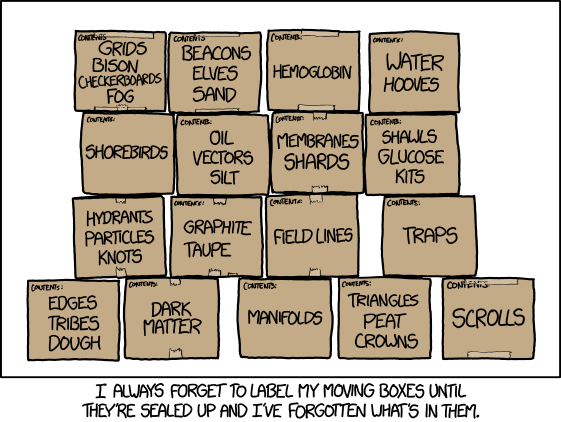
\includegraphics[width=.9\columnwidth]{res/xkcd/1762_moving_boxes.png}
}{\url{https://xkcd.com/1762}}

\fibelsig{Andreas G., Alex }
\end{multicols*}
